\documentclass[11pt,pdf,hyperref={unicode}]{beamer}
%\usetheme{boxes}
\beamertemplatenavigationsymbolsempty
\setbeamertemplate{footline}[page number]

\usepackage[utf8]{inputenc}
%\usepackage[english, russian]{babel}
\usepackage{bm}
\usepackage{multirow}
\usepackage{ragged2e}
\usepackage{indentfirst}
\usepackage{multicol}
\usepackage{subfig}
\usepackage{amsmath,amssymb}
\usepackage{enumerate}
\usepackage{mathtools}
\usepackage{comment}
\usepackage[all]{xy}
\usepackage{tikz}
\usetikzlibrary{positioning,arrows}
\tikzstyle{name} = [parameters]
\definecolor{name}{rgb}{0.5,0.5,0.5}

% colors
\definecolor{darkgreen}{rgb}{0.0, 0.2, 0.13}
\definecolor{darkcyan}{rgb}{0.0, 0.55, 0.55}

%----------------------------------------------------------------------------------------------------------

%\title{MKNBL: Joint multi-channel knowledge-aware network and broad learning for sparse knowledge graph-based recommendation}
%\author{Kirill Shevchenko}
%\institute[]{Higher School of Economics}
%\date{2024}

%---------------------------------------------------------------------------------------------------------
\begin{document}
    \begin{frame}{Sparse knowledge graph-based recommendations}
        Recommendation systems are key for providing personalized experiences, but sparse data presents a significant challenge.

        \begin{block}{The problem}
            How to enhance recommendation accuracy using knowledge graphs techniques in sparse data scenarios?
        \end{block}

        \begin{block}{The method}
            Multi-channel Knowledge-aware Network and Broad Learning (MKNBL) – a two-stage method that integrates knowledge from
            multiple sources to improve recommendations.
        \end{block}

        \begin{block}{The solution}
            \begin{enumerate}[1]
                \item Extract rich side information from the KG using a multi-channel network.
                \item Combine enriched user and item representations using Broad Learning (BLS) to enhance feature learning.
            \end{enumerate}
        \end{block}
    \end{frame}
%----------------------------------------------------------------------------------------------------------
    \begin{frame}{Framework overview}
        \begin{columns}
            \begin{column}{0.35\textwidth}
                Why MKNBL provides better results?
                \begin{enumerate}
                    \item Rich semantic integration.
                    \item Multi-channel processing.
                    \item Efficient learning with BLS.
                    \item Improved generalization.
                \end{enumerate}
            \end{column}
            \begin{column}{0.7\textwidth}
                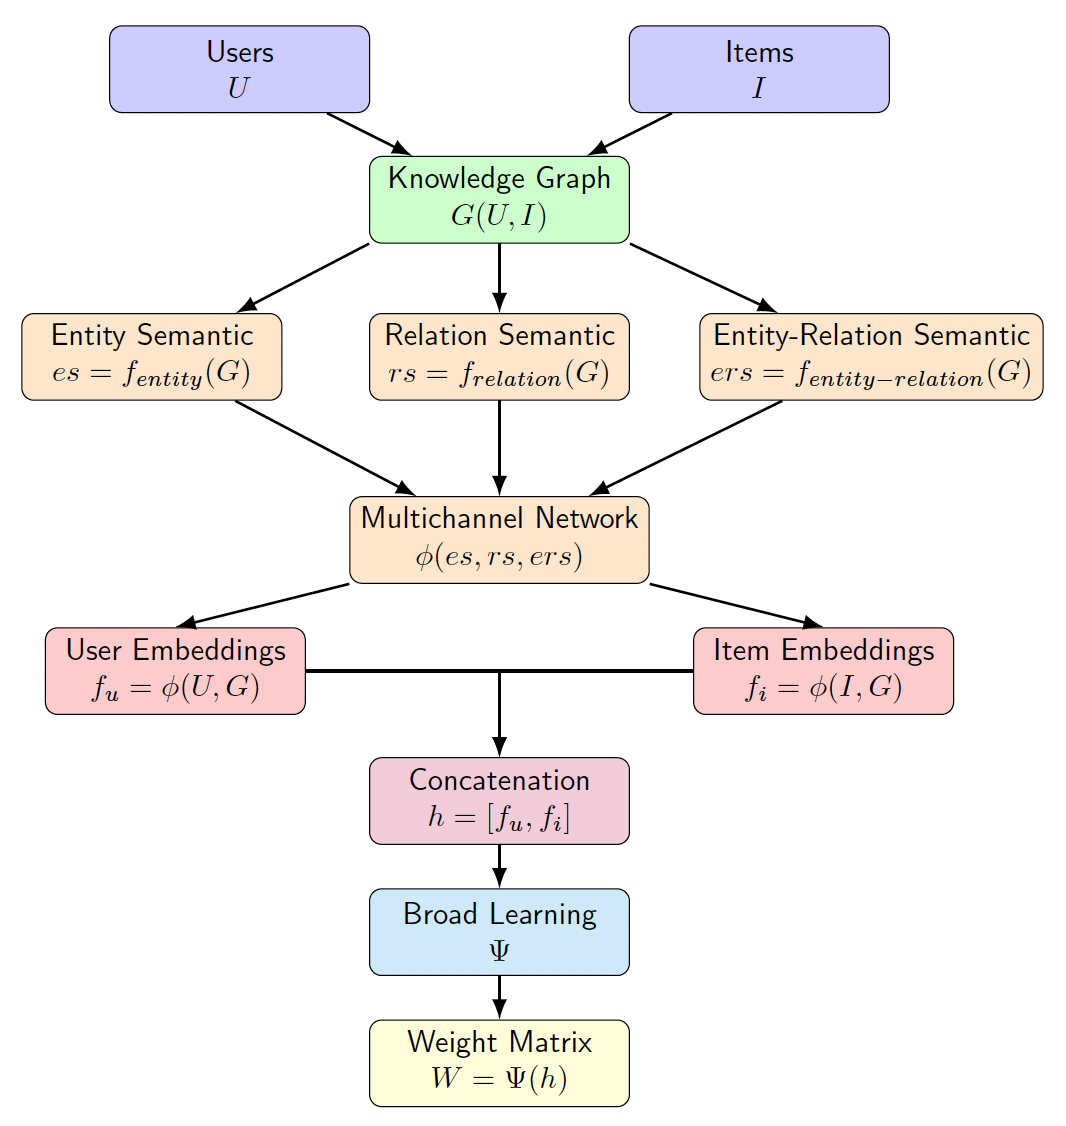
\includegraphics[width=1.0\textwidth]{Kirill-Shevchenko-Step-3-fig}      
            \end{column}
        \end{columns}
    \end{frame}
\end{document}